%
% File acl2015.tex
%
% Contact: car@ir.hit.edu.cn, gdzhou@suda.edu.cn
%%
%% Based on the style files for ACL-2014, which were, in turn,
%% Based on the style files for ACL-2013, which were, in turn,
%% Based on the style files for ACL-2012, which were, in turn,
%% based on the style files for ACL-2011, which were, in turn, 
%% based on the style files for ACL-2010, which were, in turn, 
%% based on the style files for ACL-IJCNLP-2009, which were, in turn,
%% based on the style files for EACL-2009 and IJCNLP-2008...

%% Based on the style files for EACL 2006 by 
%%e.agirre@ehu.es or Sergi.Balari@uab.es
%% and that of ACL 08 by Joakim Nivre and Noah Smith

\documentclass[11pt]{article}
\usepackage{acl2015}
\usepackage{times}
\usepackage{url}
\usepackage{latexsym}
\usepackage{graphicx}

%\setlength\titlebox{5cm}

% You can expand the titlebox if you need extra space
% to show all the authors. Please do not make the titlebox
% smaller than 5cm (the original size); we will check this
% in the camera-ready version and ask you to change it back.


\title{LSTM Recurrent Network for Step Counting based on WeAllWork Dataset}

\author{Ziyi Chen \\
  Computer Science  \\
  Unversity of California Santa Cruz\\
  {\tt zchen139@ucsc.edu}}
  
  

\date{}

\begin{document}
\maketitle
\begin{abstract}

Smartphone offers various sensors including accelerometers, gyroscope, the magnetometer that can be used for pedometer and environment-related events. This paper train an LSTM recurrent network for counting the number of steps taken by blind/sighted users, based on WeAllWork Dataset. The model is built separately for blind volunteers using long canes and guided dog as well as sighted volunteer.

\end{abstract}

\section{Introduction}

Originally used by sports and physical activity tracking, pedometers are now becoming popular as daily exercise counter and motivator. It counts each step a person takes by detecting the motion of the person's hands or hips.  Step counters can give encouragement to compete with oneself in getting fit and losing weight. Step counters are being integrated into an increasing number of portable consumer electronic devices such as music players, smartphones, and mobile phones. 

With the increasing ubiquity of smartphones, users are now carrying around a plenty of sensors like accelerometers, gyroscope, magnetometer with them wherever they go. There are various of step counting apps in smartphones. Step counters can also be used for estimating the distance and the position in indoor pedestrian navigation systems, which is especially helpful not only for blind people, but also for sighted people who need directional information in unfamiliar places.

This paper proposes an LSTM model trained by indoor walking sensor data of iPhone to predict left/right steps and calculate the count of steps. Since Blind volunteers using long canes and guided dogs as well as sighted volunteers have different features of gaits, we separately build the model and calculate the error rate of three metrics.



\section{Background and Related Work}

\subsection{Step Counting}

Automatic step counting has received substantial attention from both  research and commercial. There is a wealth of studies on the use of inertial sensors for detecting and characterising walk-related activities. Pedometer is usually portable and electronic or electromechanical. When walking, the center of gravity should be slightly moved up and down, with the most obvious upward and downward displacement of the waist. Therefore, it is most appropriate for the pedometer to be hung on the belt. It can be embedded in shoes, in a smartwatch, in a smartphone, and attached to one’s ankles or hung on the belt. 

A variety of algorithms have been proposed for stride event detection from inertial sensor time series. Some of these algorithms operate on the accelerometer data, while others use data from the gyros. For example, (WPD[7]) The Window Peak Detection algorithm runs a moving average window on the smoothed accelerometer magnitude to find peaks associated with a heel strike; (AMPD [44]) Automatic multiscale-based peak detection generic dectect peak detection in a signal; UPTIME [1]: UPTIME (Ubiquitous Pedestrian Tracking usIng Mobile phonEs) uses the de-trended magnitude of acceleration in a finite state machine (FSM), with six states to identify the peaks associated with heel strikes; HMM-acc [7][32] trains a Hidden Markov Model (HMM) to discern the different phases during a gait period; ZC-gyro [26] searches for zero crossings (ZC) within a moving window of the data from the gyro aligned with medial-lateral axis. All of the above algorithms have some parameters that must be learned from training data.

%an excellent review of some of the main algorithms is presented in [7].
Recent approaches to step detection include the use of recurrent neural networks. Researchs use RNN for evaluating and optimising accelerometer-based gesture recognition, self-calibration, pedestrian dead reckoning. Whereas the vast majority of step counting algorithms have been developed for able-bodied ambulators, some researchs have addressed the performances of these algorithms with sensors carried by people with some level of mobility impairment. 



\subsection{WeAllWalk Dataset}
WeAllWalk data set contains inertial sensor time series collected from ten blind walkers using a long cane or a guide dog and five sighted walkers. The participants walked through fairly long and complex indoor routes that included obstacles to be avoided and doors to be opened. Inertial data was recorded by iPhone 6s carried by participants in their pockets. Ground truth heel strike times were measured by two small inertial sensor units attached to the participants’ shoes. The data set contains a mobility impairment that may result in a gait pattern that is quite different than for sighted walkers. The data is subdivided into straight paths and turns and carefully annotated, with special events (or features, such as bumping into an obstacle) individually identified and marked.

\section{Implementation}
We proposes an LSTM model trained by indoor walking sensor data of iPhone to predict left/right steps and calculate the count of steps. Since Blind volunteers using long canes and guided dogs as well as sighted volunteers have different features of gaits, we separately build the model and calculate the error rate of three metrics.

\subsection{Data Preprocess}
WeAllWalk dataset contains detailed maps of indoor paths, scripts to facilitate visualization of all the information in this data set and recorded sensor data for all users and all paths.

We use two kinds of file from the dataset. First is the CSV file of iPhone sensor data as input. It contains records of all iPhone sensors. There are total 39 columns of sensor data and some of them are more useful such as rotation rate and user acceleration.

Second is the XML files that contain annotated ground truth data for all the paths walked by all the participants as labels. Each file contains start and end times for each segment the user walked through and feature information like the left or right foot as well as direction. We only train and test the step detection algorithms on data acquired while traversing straight segments in the paths, where gait is assumed to be regular, and avoided segments labeled as features. This is because the notion of “step” is not well defined in such situations. In general, we argue that step counting only really matters during regular ambulation, as an indirect way to measure distances traversed.

Since it only contains heel strike times, we cannot use it as labels directly. It is unreasonable to predict next strikes times by previous records. If we regard heel strike times as 1 and other times as 0, then the labels are unbalanced. So we apply the same sampling rate as CSV files and transform the XML file to 0-1 in which left steps as 1 and right steps as 0.

\begin{figure}[ht]
\centering
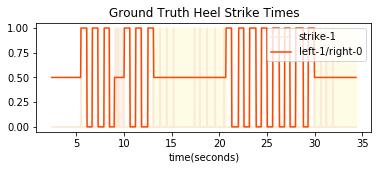
\includegraphics[scale=0.55]{ground_truth_1.png}
\caption{Example of Heel Strike Times.}
\label{fig:label}
\end{figure}

As shown in picture 1, the light color line of strike time is the origin data from XML file. It is transform to red line which regard left as 1 and right as 0. We also remove the turn data(light yellow background part) and feature data(light red backgound part).




\subsection{LSTM Model}
Long short-term memory (LSTM) network is a recurrent neural network. It can be used as blocks of recurrent neural network(RNN) network. There are different types of LSTMs, which differ in the components or connections that they have. An LSTM is suitable to predict time series such as step counting.

We use TensorFlow to implement LSTM network. TensorFlow is an open-source software library that can be used for machine learning applications such as neural networks. It supports both CPU and GPU that can be imported as a python library.

TensorFlow uses a dataflow graph to represent computation in terms of the dependencies between individual operations. We first define the dataflow graph and then create a session to run the graph. The Saver class of TensorFlow can easily add ops to save and restore variables to and from checkpoints, which map variable names to tensor values.

A two-layer RNN network with basic LSTM cell and dropout wrapper is built for training with squared difference loss function. The input is a list of metrics with the row of timesteps and col of sensor data. For Example, we want to use previous timesteps ($=50$) record of sensor data to predict the result, each sensor data contains input number ($=6$) values of rotation rate and user acceleration. So the matrix size is timesteps multiply input number($50 \times 6$). All such metrics form the input list and is transformed to tensor. Since the dataset is big and there are more than one hundred thousand elements in input list which would make the training process very slow, we divide input data into the small batch (batch size = 256) and feed the batch to model.

There are two ways of output. One is to use previous timesteps data to predict only the last step result, which is a float value around 0 to 1. We use 0.5 as the border to classify left and right steps. And the heel strike times is when 0 change to 1 or 1 change to 0. The other is to use previous timesteps data to predict corresponding timesteps step results. The first one cannot predict the first timesteps result, but it is more precise since all result is predicted by previous timesteps record.

\subsection{Error Metrics}
The round of result is a list of left/right step corresponding to origin step. Then calculate the accuracy rate of the result, which is the proportion of correct numbers (left is predicted to be left and right is predicted to be right) and total numbers.

The quality of the step counting model was measured using two different metrics. The first metric looks at the number of steps detected within each time interval separating two consecutive ground-truth heel strikes. Ideally, exactly one step should be detected within one interval. If no steps are detected in, then an undercount event is recorded. If steps are detected within that interval, the overcount events are recorded. The cumulative number of undercount and overcount events are computed and normalized (divided) by the number of ground-truth steps.

The second metric simply computes the difference between the number of detected steps within each segment and the number of ground-truth steps within the same segment. The difference between the two is recorded as an undercount value if negative, as an overcount if positive. Undercount and overcount values are then summed together over all segments, and normalized by the total number of ground-truth steps.


\section{Experience}
The model is trained with different input numbers, timesteps, output number, hidden layer number, optimizer, learning rate and training steps. We first try different optimizers with various learning rate and find that AdamOptimizer with learning rate around 0.001 can make it convergence, and then fix the two parameters.

\subsection{Blind People with Long Canes}
\subsection{Blind People with Guide Dogs}
\subsection{Sighted people}


\section{Conclusion and Future Work}

\begin{figure*}[ht]
\centering
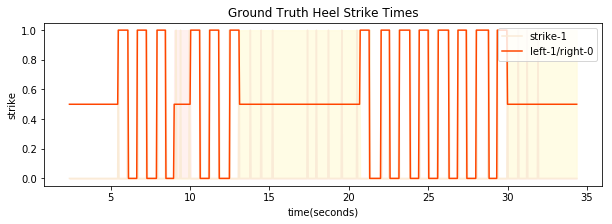
\includegraphics[scale=0.6]{ground_truth_3.png}
\caption{this is a figure demo}
\label{fig:pathdemo4}
\end{figure*}




% include your own bib file like this:
%\bibliographystyle{acl}
%\bibliography{acl2015}

\begin{thebibliography}{}

\bibitem[\protect\citename{Flores}]{Flores}
Flores, German H., and Roberto Manduchi.
\newblock (2016)
\newblock {\em WeAllWalk: An Annotated Data Set of Inertial Sensor Time Series from Blind Walkers.}.
\newblock Proceedings of the 18th International ACM SIGACCESS Conference on Computers and Accessibility. ACM, 2016.


\bibitem[\protect\citename{Brajdic}]{Brajdic}
Brajdic, Agata, and Robert Harle.
\newblock (2013)
\newblock {\em Walk detection and step counting on unconstrained smartphones.}.
\newblock Proceedings of the 2013 ACM international joint conference on Pervasive and ubiquitous computing. ACM, 2013.


\bibitem[\protect\citename{Edel}]{Brajdic}
Edel, Marcus, and Enrico Köppe.
\newblock (2015)
\newblock {\em An advanced method for pedestrian dead reckoning using BLSTM-RNNs.}.
\newblock Indoor Positioning and Indoor Navigation (IPIN), 2015 International Conference on. IEEE, 2015.



\end{thebibliography}



\end{document}





















